\begin{figure}[h!]
     \centering
    \captionsetup[sub]{font=small}
     \begin{subfigure}[b!]{0.3 \textwidth}
         \caption{}
         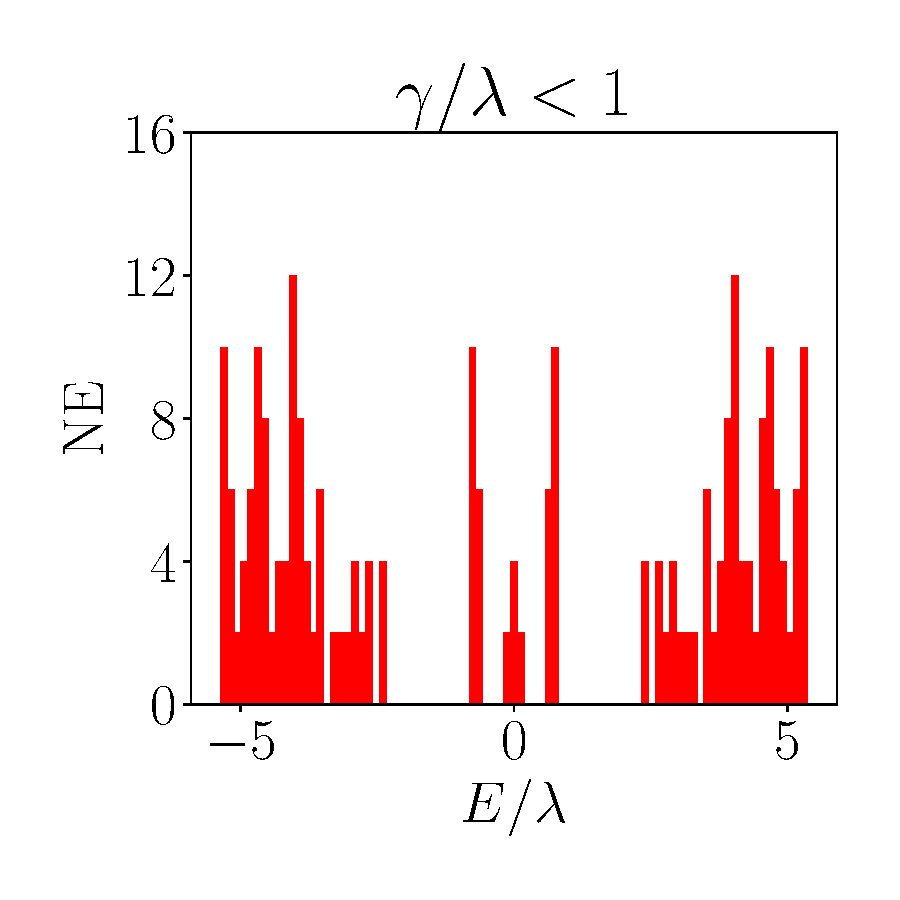
\includegraphics[width=\textwidth]{Imagenes/Resultados_Hoti_Fractal/bars_square1.pdf}
         \label{}
     \end{subfigure}\hspace*{1em}
     \begin{subfigure}[b!]{0.3 \textwidth}
         \caption{}
         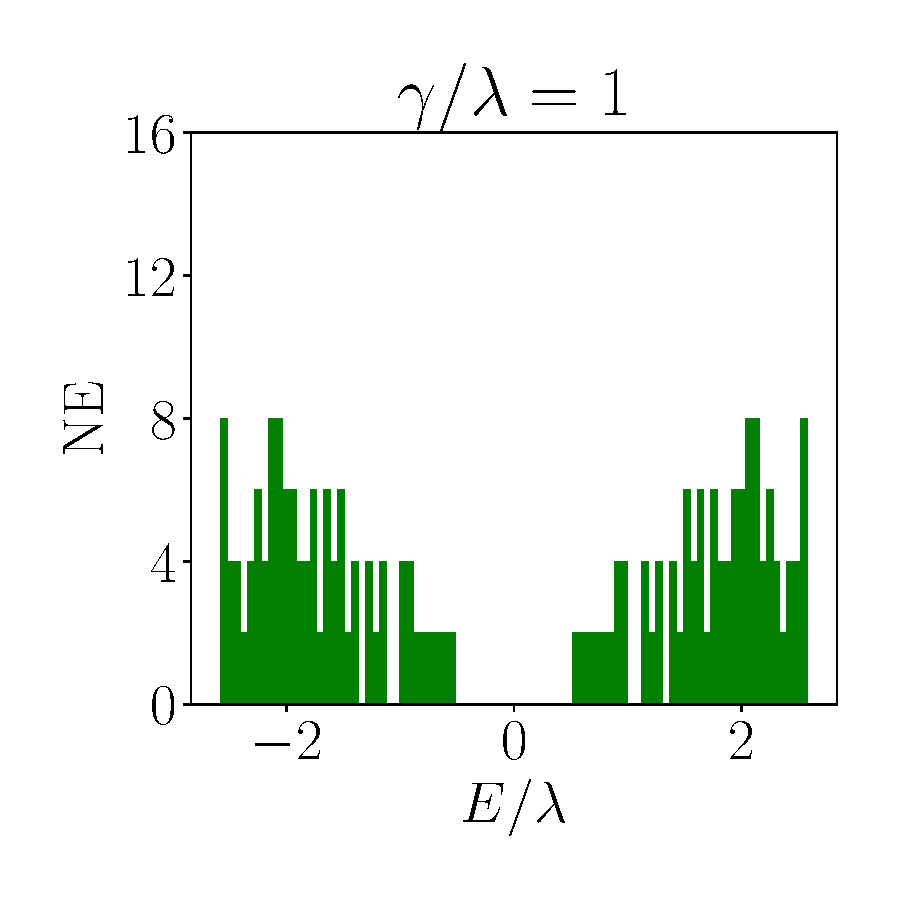
\includegraphics[width=\textwidth]{Imagenes/Resultados_Hoti_Fractal/bars_square2.pdf}
         \label{}
     \end{subfigure}\hspace*{1em}
     \begin{subfigure}[b!]{0.3 \textwidth}
         \caption{}
         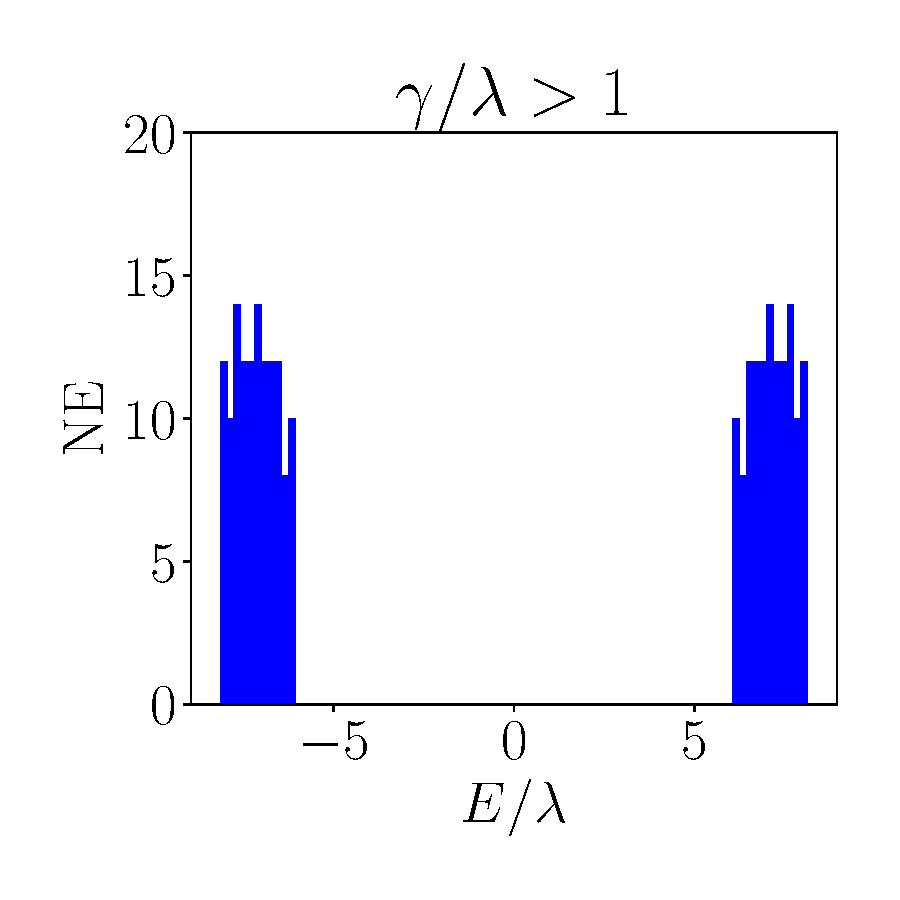
\includegraphics[width=\textwidth]{Imagenes/Resultados_Hoti_Fractal/bars_square3.pdf}
         \label{}
     \end{subfigure}\hspace*{1em}\vspace*{-1.5em}
        \caption{Cantidad de estados por energía en un red con geometría Fractal (2da generación) para diferentes valores de los parámetros de salto, \textbf{a)} $\gamma /\lambda = 1/2$, \textbf{b)} $\gamma /\lambda = 1$, \textbf{c)} $\gamma /\lambda = 2$.}
    \label{fig:Dos_fractal}
        \label{fig:Dos_Cuadrado}
\end{figure}